\documentclass[aspectratio=169]{beamer}
\usetheme{TUDelft}

% ====================================================================
% ANIMATION TOGGLE
% ====================================================================
\newif\ifanimated
\animatedtrue
\ifdefined\staticmode
  \animatedfalse
\fi
\newcommand{\cpause}{\ifanimated\pause\fi}

% Packages
\usepackage{amsmath}
\usepackage{amssymb}
\usepackage{pifont}
\usepackage{algorithm}
\usepackage{algorithmic}
\usepackage{graphicx}
\usepackage{tikz}
\usepackage{booktabs}
\usepackage{listings}
\usepackage{xcolor}
\usepackage{tcolorbox}
\usepackage{bm}

% Python code styling
\lstset{
    language=Python,
    basicstyle=\ttfamily\footnotesize,
    keywordstyle=\color{blue},
    commentstyle=\color{gray},
    stringstyle=\color{red},
    showstringspaces=false,
    breaklines=true,
    frame=single,
    numbers=left,
    numberstyle=\tiny\color{gray}
}

% TikZ libraries
\usetikzlibrary{shapes,arrows,positioning,calc,decorations.pathreplacing,fit,backgrounds,matrix}

% Import theme macros
\usepackage{tikz}
\usetikzlibrary{positioning, shapes, arrows, shadows, fit, calc, decorations.pathreplacing}

% Semantic Colors - One meaning per color
\definecolor{irSparse}{HTML}{3498DB}   % Sparse/BM25: Blue
\definecolor{irDense}{HTML}{E67E22}    % Dense/Embeddings: Orange
\definecolor{irRerank}{HTML}{C0392B}   % Rerank/Cross-encoder: Red
\definecolor{irHybrid}{HTML}{2ECC71}   % Hybrid/Fusion: Green
\definecolor{irANN}{HTML}{9B59B6}      % ANN/Infra: Purple
\definecolor{irInfra}{HTML}{58595B}    % General Infra: Dark Gray
\definecolor{irMuted}{HTML}{D9D9D9}    % Faint Gray

% Base Styles - Consistent Diagram Grammar
\tikzset{
    irBoxBase/.style={
        rectangle, 
        draw, 
        rounded corners=2pt, 
        minimum height=0.8cm, 
        minimum width=2cm,
        font=\small\sffamily,
        align=center,
        drop shadow={opacity=0.15},
        inner sep=5pt
    },
    irDatabase/.style={
        cylinder, 
        draw, 
        shape border rotate=90, 
        aspect=0.25, 
        minimum height=1.2cm, 
        minimum width=1cm,
        fill=irMuted!20,
        draw=irInfra,
        font=\tiny\sffamily,
        align=center
    },
    % Semantic Variants
    sparse/.style={irBoxBase, fill=irSparse!10, draw=irSparse},
    dense/.style={irBoxBase, fill=irDense!10, draw=irDense},
    rerank/.style={irBoxBase, fill=irRerank!10, draw=irRerank},
    hybrid/.style={irBoxBase, fill=irHybrid!10, draw=irHybrid},
    ann/.style={irBoxBase, fill=irANN!10, draw=irANN},
    infra/.style={irBoxBase, fill=irInfra!10, draw=irInfra},
    % Legacy support / Utility
    muted/.style={irBoxBase, fill=irMuted!20, draw=irMuted!80!black, text=irMuted!50!black},
    ghost/.style={irBoxBase, fill=white, draw=irMuted!50, text=irMuted, dashed, drop shadow={opacity=0}},
    emph/.style={draw=irRerank, thick, drop shadow={shadow xshift=0mm, shadow yshift=0mm, fill=irRerank, opacity=0.3}},
    % Arrows
    irArrowBase/.style={->, thick, >=latex, draw=irInfra},
    irLabel/.style={
        font=\tiny\itshape, 
        text=irInfra, 
        align=center, 
        text width=2.5cm, 
        inner sep=3pt
    }
}


% =========================================================
% Stage Badge System
% =========================================================
% \irStage{StageName}
\newcommand{\irStage}[1]{%
    \begin{tikzpicture}[remember picture, overlay]
        \node[
            anchor=north east,
            fill=irInfra!10,
            text=irInfra,
            font=\tiny\bfseries,
            inner sep=3pt,
            rounded corners=1pt,
            yshift=-0.5cm,
            xshift=-0.5cm
        ] at (current page.north east) {#1};
    \end{tikzpicture}%
}

% =========================================================
% Math Highlighting
% =========================================================
% \mathhl[color]{content}
\newcommand{\mathhl}[2][irDense!30]{%
    \colorbox{#1}{$\displaystyle #2$}%
}

% =========================================================
% Math Vectors
% =========================================================
\newcommand{\vs}{\mathbf{s}}

% =========================================================
% Core Box Primitives
% =========================================================
% \IRBox[width]{id}{at}{title}{subtitle}{variant}
% Default width chosen for lecture slides; override when needed.
% \IRBox[width]{id}{at}{title}{subtitle}{variant}[extra options]
\DeclareDocumentCommand{\IRBox}{O{3.5cm} m m m m m O{}}{%
    \node[#6, text width=#1, #7] (#2) at #3 {%
        \textbf{#4}%
        \if\relax\detokenize{#5}\relax
        \else\\[-1mm]\scriptsize #5%
        \fi
    };%
}

% \IRWideBox{id}{at}{width}{title}{subtitle}{variant}
\newcommand{\IRWideBox}[6]{%
    \node[#6, text width=#3] (#1) at #2 {%
        \textbf{#4}%
        \if\relax\detokenize{#5}\relax
        \else\\[-1mm]\scriptsize #5%
        \fi
    };%
}

% =========================================================
% Arrow Primitives
% =========================================================
% Safe default: left-to-right flow
% \IRArrow{from}{to}{label}
\newcommand{\IRArrow}[3]{%
    \draw[irArrowBase] (#1.east) -- node[irArrowLabelAbove] {#3} (#2.west);%
}

% Explicit left-to-right
% \IRArrowLR{from}{to}{label}
\newcommand{\IRArrowLR}[3]{%
    \draw[irArrowBase] (#1.east) -- node[irArrowLabelAbove] {#3} (#2.west);%
}

% Explicit top-to-bottom
% \IRArrowTB{from}{to}{label}
\newcommand{\IRArrowTB}[3]{%
    \draw[irArrowBase] (#1.south) -- node[irArrowLabelRight] {#3} (#2.north);%
}

% Fully explicit anchor-to-anchor path
% \IRArrowPath{from anchor}{to anchor}{label}
% Example: \IRArrowPath{a.east}{b.north}{score}
\newcommand{\IRArrowPath}[3]{%
    \draw[irArrowBase] (#1) -- node[irArrowLabelAbove] {#3} (#2);%
}

% Orthogonal elbow path
% \IRArrowElbow{from anchor}{to anchor}{label}
% Example: \IRArrowElbow{a.east}{b.north}{feedback}
\newcommand{\IRArrowElbow}[3]{%
    \draw[irArrowBase] (#1) -| node[irArrowLabelBox] {#3} (#2);%
}

% Slanted arrow for special cases only
% \IRArrowSlanted{from anchor}{to anchor}{label}{pos}{width}
\newcommand{\IRArrowSlanted}[5]{%
    \draw[irArrowBase] (#1) -- node[above, sloped, irLabel, pos=#4, text width=#5, fill=white, inner sep=1pt] {#3} (#2);%
}

% =========================================================
% Accent Elements
% =========================================================
% \IRBadge{at}{text}
\newcommand{\IRBadge}[2]{%
    \node[
        draw=irAccent,
        fill=irAccent!20,
        rounded corners=1pt,
        font=\tiny\bfseries,
        inner sep=2pt
    ] at #1 {#2};%
}

% =========================================================
% Grouping
% =========================================================
% \IRGroup{fit nodes}{label}{variant}
% Example: \IRGroup{(a)(b)(c)}{First-stage retrieval}{muted}
\newcommand{\IRGroup}[3]{%
    \node[
        irGroupBase,
        #3,
        fit=#1
    ] (group) {};
    \node[
        anchor=north west,
        font=\tiny\bfseries,
        #3
    ] at ([xshift=2pt,yshift=-2pt] group.north west) {#2};%
}

% =========================================================
% Domain-Specific Shapes
% =========================================================
% \IRDocStack{id}{at}{label}
\newcommand{\IRDocStack}[3]{%
    \node[irDocStack] (#1) at #2 {#3};%
}

% \IRDatabase{id}{at}{label}
\newcommand{\IRDatabase}[3]{%
    \node[irDatabase] (#1) at #2 {#3};%
}

% =========================================================
% Layout Helpers
% =========================================================
% \IRPipelineTier{id}{at}{text}{label}{variant}
\newcommand{\IRPipelineTier}[5]{%
    \IRBox{#1}{#2}{#3}{}{#5}[]
    \node[anchor=west, irLabel, xshift=0.5cm] at (#1.east) {#4};%
}

% \IRTelescopeTier{id}{at}{width}{text}{variant}
\newcommand{\IRTelescopeTier}[5]{%
    \node[
        irTelescopeBase,
        #5,
        minimum width=#3
    ] (#1) at #2 {#4};%
}

% \IRStep{id}{at}{title}{subtitle}{variant}
% Creates a numbered step badge left of a box.
\newcommand{\IRStep}[5]{%
    \node[
        circle,
        draw=irAccent,
        fill=irAccent!20,
        font=\tiny\bfseries,
        inner sep=2pt
    ] (#1_num) at #2 {#1};
    \node[
        #5,
        text width=3.5cm,
        right=1.5cm of #1_num
    ] (#1) {%
        \textbf{#3}%
        \if\relax\detokenize{#4}\relax
        \else\\[-1mm]\scriptsize #4%
        \fi
    };
    \draw[irArrowBase, thin] (#1_num.east) -- (#1.west);%
}


% Title information
\title[Lecture 4: Embeddings \& Re-ranking]{Representation Learning for Rankings}
\subtitle{From Bag-of-Words to Contextualized Representations}
\author{Avishek Anand}
\institute{Information Retrieval}
\date{\today}

\begin{document}

% Title slide
\begin{frame}
\titlepage
\end{frame}

\begin{frame}{Outline}
\tableofcontents
\end{frame}

% ====================================================================
% SECTION 1: FROM SPARSE TO DENSE
% ====================================================================
\section{From Sparse to Dense --- Why We Need Embeddings}

\begin{frame}[plain]
\sectionpage
\end{frame}

\begin{frame}{Recap: Where We Are}
% \irStage{BACKGROUND}
\textbf{The Bag-of-Words Legacy enables web-scale retrieval but lacks semantic depth.}

\vspace{0.8em}
\begin{itemize}
    \item \textbf{Efficiency}: Inverted indexes enable sub-second search.
    \item \textbf{Scoring}: BM25 provides a robust lexical baseline.
    \item \textbf{Expansion}: RM3 bridges some lexical gaps via feedback.
\end{itemize}\cpause

\vspace{1em}
\begin{alertblock}{The Persistent Problem}
Methods rely on \textbf{exact term matches}:
\begin{itemize}
    \item No semantics: \textit{car problems} $\neq$ \textit{automobile issues}.
    \item Polysemy: \textit{bank} (financial) = \textit{bank} (river).
\end{itemize}
\end{alertblock}
\end{frame}

\begin{frame}{The Representation Gap}
% \irStage{BACKGROUND}
\textbf{Lexical matching requires exact term overlap to estimate relevance.}

\vspace{0.8em}
\begin{itemize}
    \item \textbf{Sparse}: Each dimension corresponds to a vocabulary word.
    \item \textbf{Dense}: Dimensions represent latent semantic features.
    \item \textbf{Goal}: Learn embeddings where closeness $\approx$ same meaning.
\end{itemize}\cpause

\vspace{0.5em}
\begin{center}
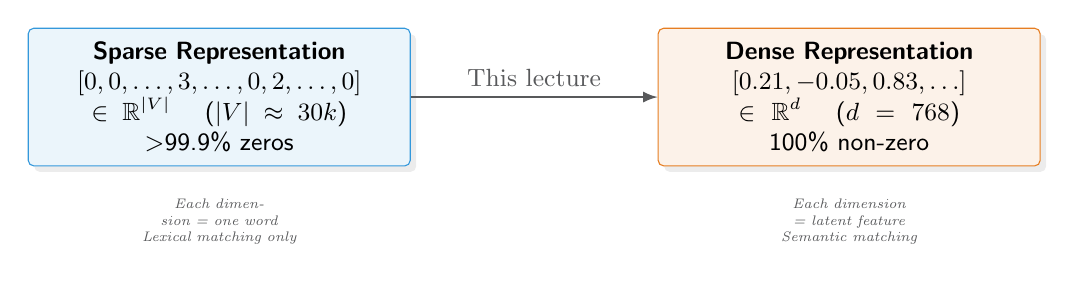
\begin{tikzpicture}
    \node[sparse, text width=4.5cm] (sparse) at (0,0) {\textbf{Sparse Representation}\\
    $[0, 0, \ldots, 3, \ldots, 0, 2, \ldots, 0]$\\
    $\in \mathbb{R}^{|V|}$ \quad ($|V| \approx 30k$)\\
    $>$99.9\% zeros};

    \node[dense, text width=4.5cm] (dense) at (8,0) {\textbf{Dense Representation}\\
    $[0.21, -0.05, 0.83, \ldots]$\\
    $\in \mathbb{R}^{d}$ \quad ($d = 768$)\\
    100\% non-zero};

    \draw[irArrowBase] (sparse) -- (dense) node[midway, above, font=\small, text=irInfra] {This lecture};

    \node[below=0.3cm of sparse, irLabel] {Each dimension = one word\\Lexical matching only};
    \node[below=0.3cm of dense, irLabel] {Each dimension = latent feature\\Semantic matching};
\end{tikzpicture}

\end{center}
\end{frame}

\begin{frame}{The Distributional Hypothesis}
% \irStage{BACKGROUND}
\begin{block}{Core Principle (Firth, 1957)}
``You shall know a word by the company it keeps.''
\end{block}

\vspace{1em}\cpause
\textbf{Example:} What is a ``\textit{tezguino}''?
\begin{itemize}
    \item ``A bottle of \textit{tezguino} is on the table.''
    \item ``Everybody enjoys \textit{tezguino}.''
    \item ``We brew \textit{tezguino} from corn.''
\end{itemize}

\cpause
\vspace{0.5em}
\textbf{Inference:} It's an alcoholic drink. Context reveals meaning!
\end{frame}

\begin{frame}{Word2Vec: Words as Vectors}
% \irStage{BACKGROUND}
\textbf{The Skip-gram model learns word meaning from local context windows.}

\vspace{0.8em}
\begin{itemize}
    \item \textbf{Hypothesis}: Words in similar contexts have similar meanings.
    \item \textbf{Task}: Predict surrounding context tokens from a target word.
    \item \textbf{Objective}: Weights in the hidden layer become the embeddings.
\end{itemize}\cpause

\vspace{0.5em}
\begin{center}
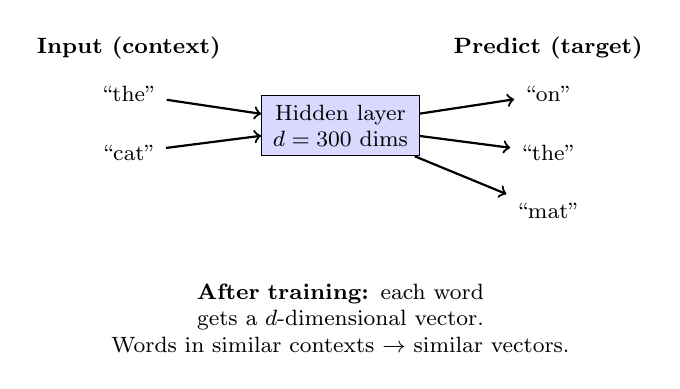
\begin{tikzpicture}[
    node distance=0.8cm,
    box/.style={rectangle, draw, minimum width=2cm, minimum height=0.6cm, font=\footnotesize, align=center},
    arrow/.style={->, thick}
]
    \node[font=\footnotesize] (ctx1) {``the''};
    \node[font=\footnotesize, below=0.3cm of ctx1] (ctx2) {``cat''};
    \node[box, fill=blue!15, right=1.2cm of ctx1, yshift=-0.4cm] (hidden) {Hidden layer\\$d = 300$ dims};
    \node[font=\footnotesize, right=1.2cm of hidden, yshift=0.4cm] (out1) {``on''};
    \node[font=\footnotesize, below=0.3cm of out1] (out2) {``the''};
    \node[font=\footnotesize, below=0.3cm of out2] (out3) {``mat''};

    \draw[arrow] (ctx1) -- (hidden);
    \draw[arrow] (ctx2) -- (hidden);
    \draw[arrow] (hidden) -- (out1);
    \draw[arrow] (hidden) -- (out2);
    \draw[arrow] (hidden) -- (out3);

    \node[above=0.1cm of ctx1, font=\footnotesize\bfseries] {Input (context)};
    \node[above=0.1cm of out1, font=\footnotesize\bfseries] {Predict (target)};

    \node[below=1.5cm of hidden, font=\footnotesize, text width=7cm, align=center] {
    \textbf{After training:} each word gets a $d$-dimensional vector.\\
    Words in similar contexts $\to$ similar vectors.};
\end{tikzpicture}

\end{center}
\end{frame}

\begin{frame}{Word2Vec: Semantic Properties}
% \irStage{BACKGROUND}
\begin{alertblock}{Semantic Properties}
$\vec{\text{king}} - \vec{\text{man}} + \vec{\text{woman}} \approx \vec{\text{queen}}$
\end{alertblock}

\vspace{1em}
\cpause
\textbf{Why this matters for IR:}
\begin{itemize}
    \item Vectors capture \textbf{relational structure}.
    \item Semantic similarity $\approx$ vector proximity (cosine similarity).
\end{itemize}
\end{frame}


\begin{frame}{Word2Vec: Relevance to IR}
% \irStage{BACKGROUND}
\textbf{Vector proximity enables matching beyond exact keywords.}

\vspace{0.8em}
\begin{itemize}
    \item \textbf{High Sim}: $\cos(\vec{\text{car}}, \vec{\text{automobile}}) \approx 0.7$.
    \item \textbf{Low Sim}: $\cos(\vec{\text{car}}, \vec{\text{banana}}) \approx 0.1$.
    \item \textbf{Recall}: Enables finding relevant docs with zero term overlap.
\end{itemize}

\vspace{1em}
\cpause

\textbf{The Naive Approach:} $\vec{d} = \frac{1}{|d|}\sum_{w \in d} \vec{w}$

\vspace{1em}
\cpause
\begin{itemize}
    \item \textbf{Mechanism:} ``the cat sat on the mat'' $\to \text{Avg}(\vec{\text{the}}, \vec{\text{cat}}, \ldots)$
    \item \textbf{Pros:} Simple, fast, significantly better than BoW for vocabulary mismatch.
\end{itemize}

\end{frame}

\begin{frame}{Query Processing with Word Embeddings}
% \irStage{BACKGROUND}
\textbf{How can we build an IR system using word embeddings?}

\cpause
\begin{itemize}
    \item \textbf{Approach}: Represent both the query $q$ and the document $d$ as vectors in the same $d$-dimensional space.
    \item \textbf{Mechanism}: Use a pre-trained \textbf{embedding table} to look up vectors for each word.
\end{itemize}

\begin{center}
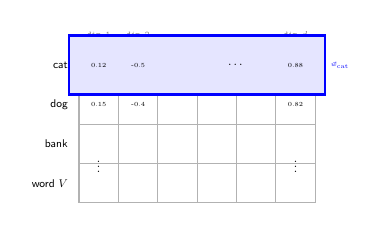
\begin{tikzpicture}[scale=0.45, transform shape,
    cell/.style={rectangle, draw=black!30, minimum size=5mm, inner sep=0pt},
    matrix label/.style={font=\small\sffamily},
    dim label/.style={font=\scriptsize\ttfamily, color=gray},
    highlight/.style={draw=blue, fill=blue!10, thick}
]

% Matrix of embeddings
\matrix (m) [matrix of nodes, nodes={cell}, column sep=-\pgflinewidth, row sep=-\pgflinewidth, nodes in empty cells] {
    & & & & & \\
    & & & & & \\
    & & & & & \\
    & & & & & \\
};

% Labels for dimensions (top)
\node[dim label, above=2pt] at (m-1-1.north) {dim 1};
\node[dim label, above=2pt] at (m-1-2.north) {dim 2};
\node[dim label, above=2pt] at (m-1-6.north) {dim $d$};

% Labels for vocabulary (left)
\node[matrix label, left=5pt] at (m-1-1.west) {cat};
\node[matrix label, left=5pt] at (m-2-1.west) {dog};
\node[matrix label, left=5pt] at (m-3-1.west) {bank};
\node[matrix label, left=5pt] at (m-4-1.west) {word $V$};

% Highlight one row (the embedding for "cat")
\node[highlight, fit=(m-1-1) (m-1-6), label={[blue, font=\tiny]right:$\vec{w}_{\text{cat}}$}] {};

% Show some values inside the boxes
\node[font=\tiny] at (m-1-1) {0.12};
\node[font=\tiny] at (m-1-2) {-0.5};
\node[font=\tiny] at (m-1-6) {0.88};

\node[font=\tiny] at (m-2-1) {0.15};
\node[font=\tiny] at (m-2-2) {-0.4};
\node[font=\tiny] at (m-2-6) {0.82};

% Dots for ellipsis
\node at ($(m-1-3)!0.5!(m-1-6)$) {\dots};
\node at ($(m-3-1)!0.5!(m-4-1)$) {\vdots};
\node at ($(m-3-6)!0.5!(m-4-6)$) {\vdots};

\end{tikzpicture}

\end{center}\cpause

\textbf{Usage in IR:}
\begin{itemize}
    \item \textbf{Represent}: $\vec{q}$ and $\vec{d}$ are derived from word vectors (e.g., via averaging).
    \item \textbf{Rank}: Documents are ranked by vector similarity: $\text{score}(q, d) = \cos(\vec{q}, \vec{d})$.
\end{itemize}
\end{frame}

\begin{frame}{So what is the problem?}
% \irStage{BACKGROUND}
\cpause
\begin{alertblock}{The Static Vector Bottleneck}
Each word has \textbf{exactly one} vector regardless of its context.
\begin{itemize}
    \item \textit{bank} (river) = \textit{bank} (financial).
\end{itemize}
\end{alertblock}

\vspace{1em}
\cpause
\begin{alertblock}{Critical Failures}
\begin{itemize}
    \item Loses word order (``dog bites man'' = ``man bites dog'').
    \item Polysemy unresolved.
\end{itemize}
\end{alertblock}
\end{frame}


\begin{frame}{Static vs. Contextualized Embeddings}
% \irStage{BACKGROUND}
\textbf{The 2018 evolution moved IR from fixed word vectors to dynamic, context-aware representations.}

\vspace{0.8em}
\begin{itemize}
    \item \textbf{Static}: Word2Vec/GloVe assignment is fixed (ignores neighbors).
    \item \textbf{Contextualized}: BERT embeddings adapt to local word usage.
    \item \textbf{Polysemy}: Distinguishes between ``\textbf{bank}'' (finance) and ``\textbf{bank}'' (river).
\end{itemize}

\vspace{0.5em}
\begin{center}
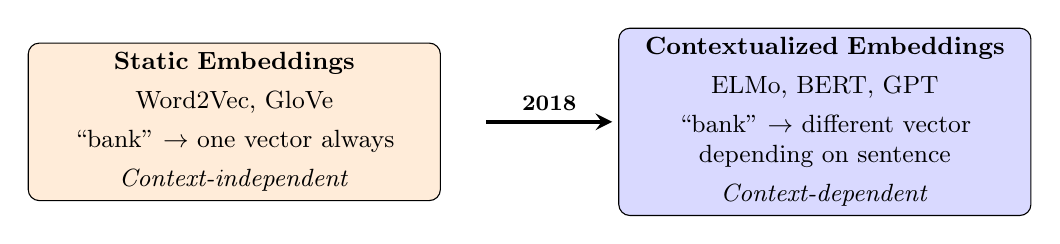
\begin{tikzpicture}[
    box/.style={rectangle, draw, rounded corners, text width=5cm, align=center, minimum height=2cm, font=\small}
]
    \node[box, fill=orange!15] (static) at (0,0) {
        \textbf{Static Embeddings}\\[3pt]
        Word2Vec, GloVe\\[3pt]
        ``bank'' $\to$ one vector always\\[3pt]
        \textit{Context-independent}
    };

    \node[box, fill=blue!15] (context) at (7.5,0) {
        \textbf{Contextualized Embeddings}\\[3pt]
        ELMo, BERT, GPT\\[3pt]
        ``bank'' $\to$ different vector\\depending on sentence\\[3pt]
        \textit{Context-dependent}
    };

    \draw[->, ultra thick, >=stealth] (3.2,0) -- (4.8,0) node[midway, above, font=\footnotesize\bfseries] {2018};
\end{tikzpicture}

\end{center}
\end{frame}

% ====================================================================
% SECTION 2: TRANSFORMERS & ATTENTION
% ====================================================================
\section{The Transformer Architecture}

\begin{frame}[plain]
\sectionpage
\end{frame}

\begin{frame}{Why Transformers?}
% \irStage{TRANSFORMERS}
\textbf{Attention mechanisms enable models to process entire sequences in parallel with global context.}

\vspace{0.8em}

They came after Recurrent Neural Networks (RNNs) and LSTMs that solved the sequence problem but were limited

\begin{itemize}
    \item \textbf{Parallelism}: Processes all tokens simultaneously (unlike sequential RNNs).
    \item \textbf{Recency}: Overcomes "forgetting" in long documents.
    \item \textbf{Scale}: Efficiently trained on massive web-scale corpora.
\end{itemize}

\vspace{1em}
\cpause
\begin{exampleblock}{The SOTA Shift}
Transformers provide the foundation for every modern high-accuracy retrieval and re-ranking system today.
\end{exampleblock}
\end{frame}

\begin{frame}[shrink=5]{Transformer Architecture}
\begin{center}

\includegraphics[width=0.35\textwidth]{figures/transformer.png}
\end{center}
\end{frame}


\begin{frame}{Self-Attention: The Core Idea}
% \irStage{TRANSFORMERS}
\textbf{Token representations are updated by "attending" to the most relevant neighbors.}

% \vspace{0.8em}
% \begin{itemize}
%     \item \textbf{Bidirectional}: Words look left and right simultaneously.
%     \item \textbf{Dynamic}: Attention weight depends on query--key similarity.
%     \item \textbf{Context}: Resolves reference (e.g., \textit{it} $\to$ \textit{animal}).
% \end{itemize}

\vspace{0.5em}
\begin{center}
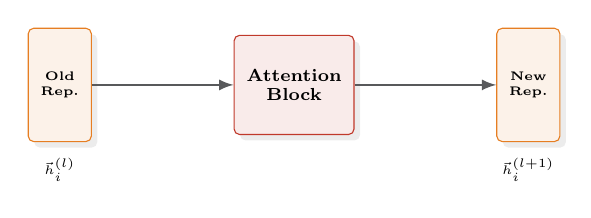
\begin{tikzpicture}[
    scale=0.9, transform shape,
    node distance=2cm,
    vector/.style={dense, minimum width=0.6cm, minimum height=1.6cm, font=\tiny\bfseries, align=center},
    block/.style={rerank, minimum size=1.4cm, font=\scriptsize\bfseries, align=center},
    arrow/.style={irArrowBase}
]

% Old representation
\node[vector] (old) at (0,0) {Old\\Rep.};
\node[below=0.1cm of old, font=\tiny] {$\vec{h}_i^{(l)}$};

% Attention Block
\node[block, right=of old] (attn) {Attention\\Block};

% New representation
\node[vector, right=of attn] (new) {New\\Rep.};
\node[below=0.1cm of new, font=\tiny] {$\vec{h}_i^{(l+1)}$};

% Arrows
\draw[arrow] (old.east) -- (attn.west);
\draw[arrow] (attn.east) -- (new.west);

\end{tikzpicture}

\end{center}

\vspace{0.8em}
\begin{center}
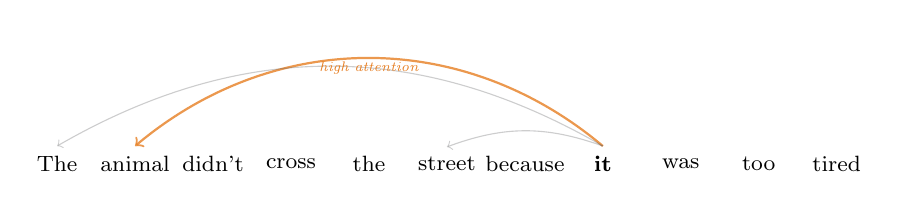
\begin{tikzpicture}[scale=0.9]
    \foreach \i/\word in {0/The, 1/animal, 2/didn't, 3/cross, 4/the, 5/street, 6/because, 7/\textbf{it}, 8/was, 9/too, 10/tired} {
        \node[font=\footnotesize] (w\i) at (\i*1.1, 0) {\word};
    }
    \draw[->, thick, irDense, opacity=0.8] (w7.north) to[bend right=40] (w1.north);
    \draw[->, thin, irInfra, opacity=0.3] (w7.north) to[bend right=30] (w0.north);
    \draw[->, thin, irInfra, opacity=0.3] (w7.north) to[bend right=20] (w5.north);
    \node[above=0.8cm of w4, irLabel, text=irDense] {high attention};
\end{tikzpicture}

\end{center}
\end{frame}

\begin{frame}{Self-Attention: The Mechanism}
% \irStage{TRANSFORMERS}
\textbf{Interaction is computed via dot-products in Query, Key, and Value spaces.}

\vspace{0.8em}
\begin{itemize}
    \item \textbf{Query} ($\vec{q}$): ``What am I looking for in other tokens?''
    \item \textbf{Key} ($\vec{k}$): ``What information do I offer to others?''
    \item \textbf{Value} ($\vec{v}$): The actual information content to be aggregated.
\end{itemize}

\vspace{1em}
\cpause
\begin{block}{The Attention Formula}
\[
\text{Attention}(Q, K, V) = \text{softmax}\left(\frac{\mathhl{QK^T}}{\sqrt{d_k}}\right) V
\]
\end{block}
\end{frame}

\begin{frame}{Breaking Down the Formula}
% \irStage{TRANSFORMERS}
\[
\text{Attention} = \text{softmax}\left(\frac{\mathhl{QK^T}}{\sqrt{d_k}}\right) V
\]
\begin{itemize}
    \item \textbf{Dot Product} ($QK^T$): Measures raw similarity between tokens.
    \item \textbf{Scaling} ($\sqrt{d_k}$): Stabilizes gradients for deep training.
    \item \textbf{Processing}: Softmax converts scores to weighting factors (sum to 1).
\end{itemize}\cpause
\end{frame}

\begin{frame}{Worked Example: Information Flow}
% \irStage{TRANSFORMERS}
\textbf{Sentence:} ``\texttt{retrieval models}'' ($d_k = 2$)

\vspace{0.5em}
\begin{enumerate}
    \item \textbf{Similarity}: $\vec{q}_{\text{retr}} \cdot \vec{k}_{\text{retr}} = 0.9$ (Self) \quad $\vec{q}_{\text{retr}} \cdot \vec{k}_{\text{mod}} = 0.6$ (Neighbor)
    \cpause
    \item \textbf{Weights}: $\text{softmax}([0.9, 0.6]) \approx [\,\mathhl{0.57},\; \mathhl{0.43}\,]$
    \cpause
    \item \textbf{Output}: $\vec{h}_{\text{retr}} = 0.57 \vec{v}_{\text{retr}} + 0.43 \vec{v}_{\text{mod}}$
\end{enumerate}

\vspace{1em}
\cpause
\begin{exampleblock}{Interpretation}
The representation of ``retrieval'' is now updated with 43\% of the information from ``models''. Context is integrated!
\end{exampleblock}
\end{frame}

\begin{frame}{Multi-Head Attention}
% \irStage{TRANSFORMERS}
\textbf{Parallel attention heads learn different linguistic and semantic relationships.}

\vspace{0.8em}
\begin{itemize}
    \item \textbf{Heads}: BERT uses 8 heads per layer in parallel.
    \item \textbf{Variety}: Heads learn distinct features (Syntax, Entities, etc.).
    \item \textbf{Robustness}: Aggregating heads provides a richer representation.
\end{itemize}

\vspace{1em}
\cpause
\begin{exampleblock}{Feature Extraction}
Calculates 8 different embeddings per token, then concatenates them.
\end{exampleblock}
\end{frame}

\begin{frame}{Positional Encoding}
% \irStage{TRANSFORMERS}
\textbf{Since attention is permutation-invariant, we must inject word order manually.}

\vspace{0.8em}
\begin{itemize}
    \item \textbf{Problem}: Without positions, \textit{dog bites man} = \textit{man bites dog}.
    \item \textbf{Solution}: Add a unique position vector $\vec{p}_i$ to each token $\vec{e}_i$.
    \item \textbf{Result}: Model learns both identity and relative location.
\end{itemize}

\vspace{1em}
\cpause
\begin{block}{Combined Input Representation}
\[
\vec{x}_i = \vec{e}_{\text{word}_i} + \vec{p}_i
\]
\end{block}
\end{frame}

\begin{frame}{The Transformer Encoder Block}
% \irStage{TRANSFORMERS}
\textbf{Each encoder block combines parallel attention with per-token feed-forward processing.}

\vspace{0.8em}
\begin{columns}
\begin{column}{0.5\textwidth}
\begin{itemize}
    \item \textbf{Attention}: Token interaction via Q, K, V.
    \item \textbf{Residuals}: Prevents gradient signal decay.
    \item \textbf{Norm}: Stabilizes flow through deep layers.
\end{itemize}\cpause

% \begin{block}{BERT Base Spec}
% \begin{itemize}
%     \item 12 Layers / 768 Dimensions
%     \item 12 Heads / 110M Params
% \end{itemize}
% \end{block}
\end{column}

\begin{column}{0.45\textwidth}
\begin{center}
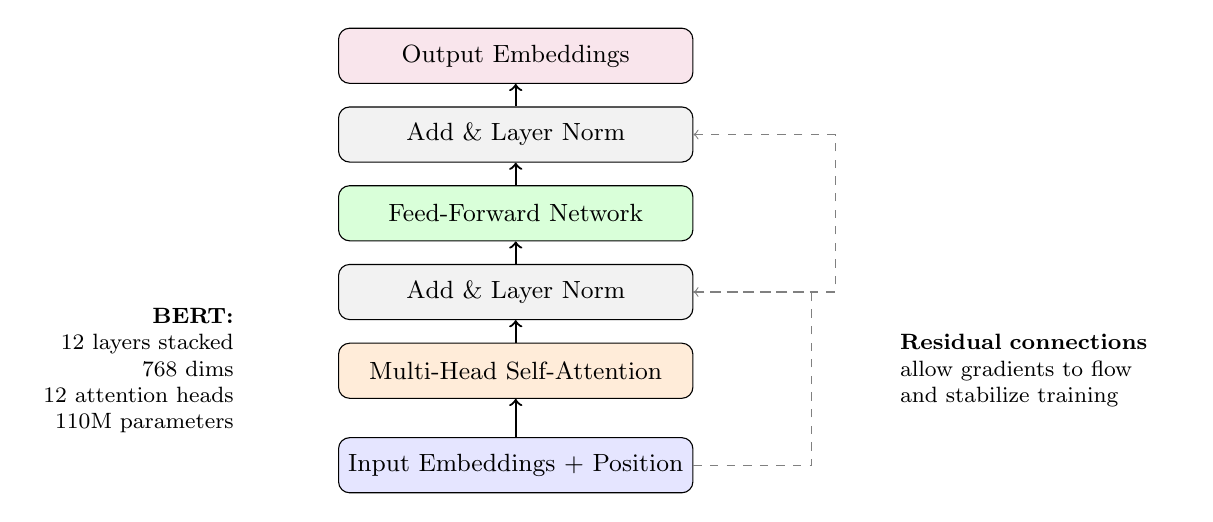
\begin{tikzpicture}[
    block/.style={rectangle, draw, rounded corners, minimum width=4.5cm, minimum height=0.7cm, align=center, font=\small},
    arrow/.style={->, thick}
]
    \node[block, fill=blue!10] (input) at (0, 0) {Input Embeddings + Position};
    \node[block, fill=orange!15] (attn) at (0, 1.2) {Multi-Head Self-Attention};
    \node[block, fill=gray!10] (add1) at (0, 2.2) {Add \& Layer Norm};
    \node[block, fill=green!15] (ffn) at (0, 3.2) {Feed-Forward Network};
    \node[block, fill=gray!10] (add2) at (0, 4.2) {Add \& Layer Norm};
    \node[block, fill=purple!10] (out) at (0, 5.2) {Output Embeddings};

    \draw[arrow] (input) -- (attn);
    \draw[arrow] (attn) -- (add1);
    \draw[arrow] (add1) -- (ffn);
    \draw[arrow] (ffn) -- (add2);
    \draw[arrow] (add2) -- (out);

    % Residual connections
    \draw[->, dashed, gray] (input.east) -- ++(1.5,0) |- (add1.east);
    \draw[->, dashed, gray] (add1.east) -- ++(1.8,0) |- (add2.east);

    \node[right=2.5cm of attn, text width=3.5cm, font=\footnotesize] {
        \textbf{Residual connections}\\
        allow gradients to flow\\
        and stabilize training
    };

    \node[left=1.2cm of attn, font=\footnotesize, text width=2.5cm, align=right] {
        \textbf{BERT:}\\
        12 layers stacked\\
        768 dims\\
        12 attention heads\\
        110M parameters
    };
\end{tikzpicture}

\end{center}
\end{column}
\end{columns}
\end{frame}


% ====================================================================
% SECTION 3: BERT FOR IR
% ====================================================================
\section{BERT for Information Retrieval}

\begin{frame}[plain]
\sectionpage
\end{frame}

\begin{frame}[shrink=5]{What is BERT?}
% \irStage{BERT}
\textbf{BERT (Bidirectional Encoder Representations from Transformers) is an encoder-only model.}

\vspace{0.8em}
\begin{columns}
\begin{column}{0.55\textwidth}
\begin{itemize}
    \item \textbf{Encoder vs.\ Generative}:
    \begin{itemize}
        \item \textbf{Generative (e.g., GPT)}: Causal; predicts the next token.
        \item \textbf{Encoder (BERT)}: Bidirectional; sees the entire sequence simultaneously.
    \end{itemize}
    \item \textbf{Context Aware}: Embeddings are computed based on \textbf{all} surrounding tokens.
    \item \textbf{Instance}: BERT is a specific implementation of a Transformer Encoder.
\end{itemize}
\end{column}

\begin{column}{0.4\textwidth}
\begin{center}

\includegraphics[width=\textwidth]{figures/bert}\\
\scriptsize \textbf{Encoder Representation}
\end{center}
\end{column}
\end{columns}
\end{frame}

\begin{frame}{BERT Architecture: Core Components}
% \irStage{BERT}
\textbf{The BERT architecture consists of three fundamental layers of processing.}

\vspace{0.8em}
\begin{enumerate}
    \item \textbf{Embeddings Layer}:
    \begin{itemize}
        \item \textbf{BPE / WordPiece}: Splits tokens into sub-words (e.g., \textit{embedding} $\to$ \textit{embed}, \textit{\#\#ding}).
        \item \textbf{Positional Encoding}: Injects sequence order info.
    \end{itemize}\cpause
    \item \textbf{Multi-Head Attention (MHA)}:
    \begin{itemize}
        \item Computes token interactions via Q, K, V dot-products.
        \item Every token "attends" to every other token in the sequence.
    \end{itemize}\cpause
    \item \textbf{Stacking \& Residuals}:
    \begin{itemize}
        \item Stacks many identical encoder blocks (12 for Base, 24 for Large).
        \item \textbf{Residual Stream}: Skip-connections allow signal to flow across layers.
    \end{itemize}
\end{enumerate}
\end{frame}

\begin{frame}{Step 1: Subword Tokenization}
% \irStage{BERT}
\textbf{BERT processes text by breaking words into frequent sub-words (WordPiece).}

\vspace{0.8em}
\begin{itemize}
    \item \textbf{Query}: ``how to rank'' $\to$ \texttt{[how, to, rank]}
    \item \textbf{Doc}: ``ranking models'' $\to$ \texttt{[rank, \#\#ing, models]}
    \item \textbf{Sequence}: \texttt{[CLS] Q [SEP] D [SEP]}
\end{itemize}

\vspace{1.5em}
\cpause
\begin{block}{The Input Sequence}
\begin{center}
\texttt{[\mathhl{CLS}] how to rank [\mathhl{SEP}] rank \#\#ing models [\mathhl{SEP}]}
\end{center}
\end{block}
\end{frame}

\begin{frame}[shrink=5]{Step 2: Combining Embeddings}
% \irStage{BERT}
\textbf{The model must know where tokens are and which sequence they belong to.}

\vspace{1em}
\begin{center}
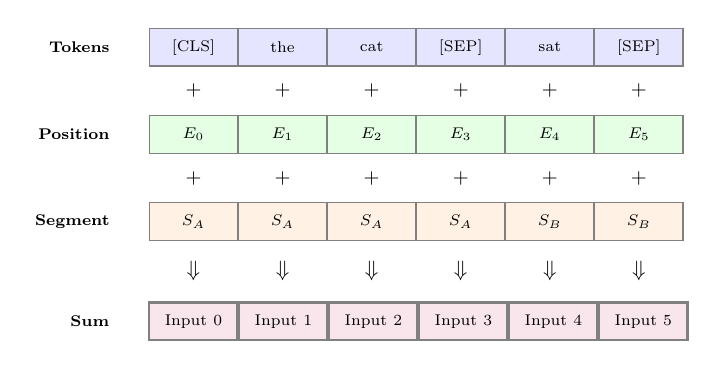
\begin{tikzpicture}[
    scale=0.8, transform shape,
    node distance=0cm,
    box/.style={rectangle, draw=black!50, minimum width=1.4cm, minimum height=0.6cm, font=\scriptsize, align=center},
    plus/.style={font=\small, inner sep=2pt},
    token/.style={fill=blue!10},
    posE/.style={fill=green!10},
    seg/.style={fill=orange!10},
    sum/.style={fill=purple!10, thick}
]

% Tokens
\node[box, token] (t0) {[CLS]};
\node[box, token, right=of t0] (t1) {the};
\node[box, token, right=of t1] (t2) {cat};
\node[box, token, right=of t2] (t3) {[SEP]};
\node[box, token, right=of t3] (t4) {sat};
\node[box, token, right=of t4] (t5) {[SEP]};

\node[left=0.5cm of t0, font=\scriptsize\bfseries] {Tokens};

% Plus sign 1
\node[plus, below=0.2cm of t0] (p1) {+};
\node[plus, below=0.2cm of t1] {+};
\node[plus, below=0.2cm of t2] {+};
\node[plus, below=0.2cm of t3] {+};
\node[plus, below=0.2cm of t4] {+};
\node[plus, below=0.2cm of t5] {+};

% Position Embeddings
\node[box, posE, below=0.2cm of p1] (pos0) {$E_0$};
\node[box, posE, right=of pos0] (pos1) {$E_1$};
\node[box, posE, right=of pos1] (pos2) {$E_2$};
\node[box, posE, right=of pos2] (pos3) {$E_3$};
\node[box, posE, right=of pos3] (pos4) {$E_4$};
\node[box, posE, right=of pos4] (pos5) {$E_5$};

\node[left=0.5cm of pos0, font=\scriptsize\bfseries] {Position};

% Plus sign 2
\node[plus, below=0.2cm of pos0] (p2) {+};
\node[plus, below=0.2cm of pos1] {+};
\node[plus, below=0.2cm of pos2] {+};
\node[plus, below=0.2cm of pos3] {+};
\node[plus, below=0.2cm of pos4] {+};
\node[plus, below=0.2cm of pos5] {+};

% Segment Embeddings
\node[box, seg, below=0.2cm of p2] (seg0) {$S_A$};
\node[box, seg, right=of seg0] (seg1) {$S_A$};
\node[box, seg, right=of seg1] (seg2) {$S_A$};
\node[box, seg, right=of seg2] (seg3) {$S_A$};
\node[box, seg, right=of seg3] (seg4) {$S_B$};
\node[box, seg, right=of seg4] (seg5) {$S_B$};

\node[left=0.5cm of seg0, font=\scriptsize\bfseries] {Segment};

% Equal sign
\node[below=0.2cm of seg0] (eq) {$\Downarrow$};
\node[below=0.2cm of seg1] {$\Downarrow$};
\node[below=0.2cm of seg2] {$\Downarrow$};
\node[below=0.2cm of seg3] {$\Downarrow$};
\node[below=0.2cm of seg4] {$\Downarrow$};
\node[below=0.2cm of seg5] {$\Downarrow$};

% Final Input
\node[box, sum, below=0.2cm of eq] (in0) {Input 0};
\node[box, sum, right=of in0] (in1) {Input 1};
\node[box, sum, right=of in1] (in2) {Input 2};
\node[box, sum, right=of in2] (in3) {Input 3};
\node[box, sum, right=of in3] (in4) {Input 4};
\node[box, sum, right=of in4] (in5) {Input 5};

\node[left=0.5cm of in0, font=\scriptsize\bfseries] {Sum};

\end{tikzpicture}

\end{center}

\vspace{0.5em}
\cpause
\begin{itemize}
    \item \textbf{Token}: The sub-word ID from the vocabulary.
    \item \textbf{Position}: A unique vector for index $0, 1, 2, \ldots$
    \item \textbf{Segment}: $S_A$ for Query, $S_B$ for Document.
\end{itemize}
\end{frame}

\begin{frame}{Step 3: Transformer Stacking to [CLS]}
% \irStage{BERT}
\textbf{The [CLS] token aggregates context from the entire (q, d) pair.}

\vspace{0.8em}
\begin{columns}
\begin{column}{0.45\textwidth}
\begin{itemize}
    \item \textbf{Transformation}: Each layer updates all token representations.
    \item \textbf{Context}: Through MHA, the \texttt{[CLS]} vector "sees" the relationship between query and doc.
    \item \textbf{Pooling}: The final vector at index 0 becomes our representation.
\end{itemize}
\end{column}

\begin{column}{0.5\textwidth}
\begin{center}
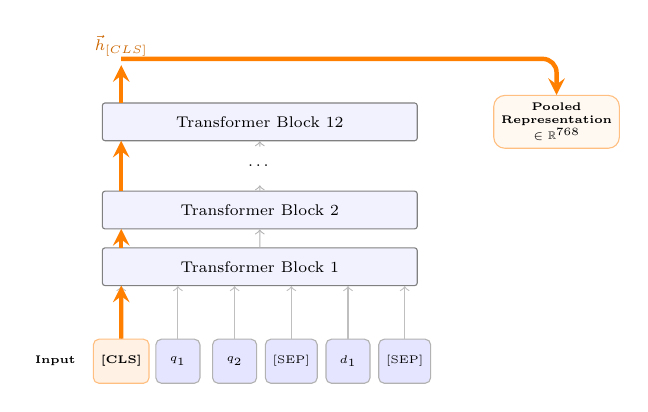
\begin{tikzpicture}[
    scale=0.8, transform shape,
    block/.style={rectangle, draw=black!50, fill=blue!5, minimum width=5cm, minimum height=0.6cm, font=\scriptsize, align=center, rounded corners=1pt},
    token/.style={rectangle, draw=black!30, fill=blue!10, minimum size=0.7cm, font=\tiny, rounded corners=2pt},
    cls_token/.style={rectangle, draw=orange!50, fill=orange!10, minimum size=0.7cm, font=\tiny\bfseries, rounded corners=2pt},
    cls_path/.style={orange, ultra thick, ->, >=stealth}
]

% Input tokens
\node[cls_token] (t0) at (-2.2, -1.5) {[CLS]};
\node[token] (t1) at (-1.3, -1.5) {$q_1$};
\node[token] (t2) at (-0.4, -1.5) {$q_2$};
\node[token] (t3) at (0.5, -1.5) {[SEP]};
\node[token] (t4) at (1.4, -1.5) {$d_1$};
\node[token] (t5) at (2.3, -1.5) {[SEP]};

\node[anchor=east, font=\tiny\bfseries] at (-2.8, -1.5) {Input};

% Transformer blocks
\node[block] (b1) at (0, 0) {Transformer Block 1};
\node[block] (b2) at (0, 0.9) {Transformer Block 2};
\node[block, fill=none, draw=none] (dots) at (0, 1.6) {\dots};
\node[block] (b12) at (0, 2.3) {Transformer Block 12};

% Base arrows from tokens to Block 1
\foreach \i in {0,...,5} {
    \draw[->, gray!50, thin] (t\i.north) -- (t\i.north |- b1.south);
}

% Arrows between blocks
\draw[->, gray!60] (b1) -- (b2);
\draw[->, gray!60] (b2) -- (dots);
\draw[->, gray!60] (dots) -- (b12);

% Highlight CLS path (through the layers)
\draw[cls_path] (t0.north) -- (-2.2, -0.3);
\draw[cls_path] (-2.2, 0.3) -- (-2.2, 0.6);
\draw[cls_path] (-2.2, 1.2) -- (-2.2, 2.0);
\draw[cls_path] (-2.2, 2.6) -- (-2.2, 3.2) node[above, font=\scriptsize\bfseries, color=orange!80!black] {$\vec{h}_{[CLS]}$};

% Pooling to Vector
\node[draw=orange!50, fill=orange!5, rounded corners, right=1.2cm of b12, align=center, font=\tiny\bfseries] (vec) {Pooled\\Representation\\$\in \mathbb{R}^{768}$};

\draw[cls_path, rounded corners=5pt] (-2.2, 3.3) -| (vec.north);

\end{tikzpicture}

\end{center}
\end{column}
\end{columns}
\end{frame}

\begin{frame}{Alternative: Token-wise Representations}
% \irStage{BERT}
\textbf{BERT also provides a contextualized vector for every single input token.}

\vspace{0.8em}
\begin{columns}
\begin{column}{0.45\textwidth}
\begin{itemize}
    \item \textbf{Rich Context}: Each $\vec{h}_i$ contains the meaning of token $i$ *in that specific sequence*.
    \item \textbf{Applications}:
        \begin{itemize}
            \item \textbf{NER/POS}: Classify each token.
            \item \textbf{Question Answering}: Predict start/end spans.
            \item \textbf{Late Interaction}: Used in models like ColBERT.
        \end{itemize}
\end{itemize}
\end{column}

\begin{column}{0.5\textwidth}
\begin{center}
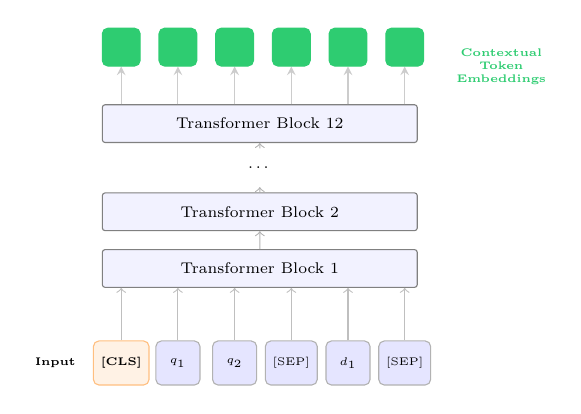
\begin{tikzpicture}[
    scale=0.8, transform shape,
    block/.style={rectangle, draw=black!50, fill=blue!5, minimum width=5cm, minimum height=0.6cm, font=\scriptsize, align=center, rounded corners=1pt},
    token/.style={rectangle, draw=black!30, fill=blue!10, minimum size=0.7cm, font=\tiny, rounded corners=2pt},
    cls_token/.style={rectangle, draw=orange!50, fill=orange!10, minimum size=0.7cm, font=\tiny\bfseries, rounded corners=2pt},
    h_node/.style={rectangle, draw=irHybrid!50, fill=irHybrid!10, minimum size=0.6cm, font=\tiny, rounded corners=2pt},
    out_path/.style={irHybrid, thick, ->, >=stealth}
]

% Input tokens
\node[cls_token] (t0) at (-2.2, -1.5) {[CLS]};
\node[token] (t1) at (-1.3, -1.5) {$q_1$};
\node[token] (t2) at (-0.4, -1.5) {$q_2$};
\node[token] (t3) at (0.5, -1.5) {[SEP]};
\node[token] (t4) at (1.4, -1.5) {$d_1$};
\node[token] (t5) at (2.3, -1.5) {[SEP]};

\node[anchor=east, font=\tiny\bfseries] at (-2.8, -1.5) {Input};

% Transformer blocks
\node[block] (b1) at (0, 0) {Transformer Block 1};
\node[block] (b2) at (0, 0.9) {Transformer Block 2};
\node[block, fill=none, draw=none] (dots) at (0, 1.6) {\dots};
\node[block] (b12) at (0, 2.3) {Transformer Block 12};

% Base arrows from tokens to Block 1
\foreach \i in {0,...,5} {
    \draw[->, gray!50, thin] (t\i.north) -- (t\i.north |- b1.south);
}

% Arrows between blocks
\draw[->, gray!60] (b1) -- (b2);
\draw[->, gray!60] (b2) -- (dots);
\draw[->, gray!60] (dots) -- (b12);

% Output Contextual Representations for all tokens
\foreach \i in {0,...,5} {
    \draw[out_path, gray!40, thin] (t\i.north |- b12.north) -- ++(0, 0.6) node[h_node, anchor=south, irHybrid] (h\i) {$\vec{h}_{\i}$};
}

% Label for the representations
\node[anchor=west, font=\tiny\bfseries, color=irHybrid, align=center] at (3.0, 3.2) {Contextual\\Token\\Embeddings};

\end{tikzpicture}

\end{center}
\end{column}
\end{columns}
\end{frame}

\begin{frame}{Pre-training at Scale}
% \irStage{BERT}
\textbf{BERT was the first model to leverage massive unlabeled data for general language understanding.}

\vspace{0.8em}
\begin{itemize}
    \item \textbf{The Scale Shift}: Trained on Google Books (800M words) + Wikipedia (2.5B words).
    \item \textbf{Masked LM (MLM)}: Hides 15\% of tokens to predict from context.
    \item \textbf{Next Sentence Prediction (NSP)}: Learns sequence coherence.
\end{itemize}

\vspace{1em}
\cpause
\begin{block}{The Result}
A "foundation model" that already knows how language works and stores significant \textbf{world knowledge}.
\end{block}
\end{frame}

\begin{frame}{Transfer Learning: Fine-tuning as "Orienting"}
% \irStage{BERT}
\textbf{Transfer learning allows us to adapt a foundation model to specific IR tasks.}

\vspace{0.8em}
\begin{itemize}
    \item \textbf{Pre-training}: Learns general semantics (Expensive, done once).
    \item \textbf{Fine-tuning}: The process of \textbf{"orienting"} pre-trained knowledge to a specific task (e.g., Ranking).
    \item \textbf{Efficiency}: Requires much less data and compute than training from scratch.
\end{itemize}

\vspace{0.5em}
\cpause
\begin{exampleblock}{Analogy}
A student graduating from university (Pre-training) is "fine-tuned" when they start a specific job.
\end{exampleblock}
\end{frame}

\begin{frame}{What BERT Knows: Layer by Layer}
% \irStage{BERT}
\textbf{Experiments show that BERT encodes linguistic features hierarchically.}

\vspace{0.8em}
\begin{itemize}
    \item \textbf{Lower Layers}: Surface-level NLP (POS tagging, morphology, syntax).
    \item \textbf{Middle Layers}: Complex semantics and coreference resolution.
    \item \textbf{Upper Layers}: Abstract world knowledge and task-specific logic.
\end{itemize}

\vspace{1em}
\cpause
\begin{alertblock}{For IR Ranking}
Upper layers provide the "deep" semantic matching required to bridge the lexical gap.
\end{alertblock}
\end{frame}


\begin{frame}[shrink=10]{Cross-Encoder or MonoBERT: BERT for Re-ranking}
% \irStage{RE-RANKING}
\textbf{Cross-Encoders enable deep token-level interaction between query and document.}

\vspace{0.8em}
\begin{itemize}
    \item \textbf{Input}: Feed query $q$ and document $d$ together as one sequence.
    \item \textbf{Interaction}: Every query token attends to every document token.
    \item \textbf{Scoring}: The final [CLS] token output serves as the relevance score.
\end{itemize}\cpause

\vspace{0.5em}
\begin{center}
% \begin{tikzpicture}[scale=0.8, transform shape]
    % Input tokens (generic style)
    \node[muted, compact] (cls) at (0, 0) {[CLS]};
    \node[rerank, compact, fill=irRerank!10] (q1) at (1.1, 0) {car};
    \node[rerank, compact, fill=irRerank!10] (q2) at (2.2, 0) {problems};
    \node[muted, compact] (sep1) at (3.3, 0) {[SEP]};
    \node[rerank, compact, fill=irHybrid!10, draw=irHybrid] (d1) at (4.4, 0) {auto};
    \node[rerank, compact, fill=irHybrid!10, draw=irHybrid] (d2) at (5.5, 0) {\#\#mobile};
    \node[rerank, compact, fill=irHybrid!10, draw=irHybrid] (d3) at (6.6, 0) {issues};
    \node[rerank, compact, fill=irHybrid!10, draw=irHybrid] (d4) at (7.7, 0) {and};
    \node[rerank, compact, fill=irHybrid!10, draw=irHybrid] (d5) at (8.8, 0) {fixes};
    \node[muted, compact] (sep2) at (9.9, 0) {[SEP]};

    % BERT block
    \node[rerank, minimum width=9.9cm, minimum height=1.5cm, fill=irRerank!20, thick] (bert) at (4.95, 2.2) {\textbf{BERT} (12 layers $\times$ 12 heads)\\Full cross-attention between \textcolor{irRerank}{query} and \textcolor{irHybrid}{document}};
    % Output
    \node[rerank, minimum width=1.5cm, fill=irRerank!30] (clsout) at (0, 4.5) {$h_{\text{[CLS]}}$};
    \node[rerank, minimum width=2.5cm, fill=irRerank!40] (score) at (0, 6.2) {$P(\text{rel}) = \sigma(W \cdot h_{\text{[CLS]}})$};

    % Arrows
    \foreach \n in {cls, q1, q2, sep1, d1, d2, d3, d4, d5, sep2} {
        \draw[irArrowBase, thin] (\n.north) -- (\n.north |- bert.south);
    }
    \draw[irArrowBase] (bert.north -| clsout) -- (clsout.south);
    \draw[irArrowBase] (clsout) -- (score);

    % Labels
    \node[left=0.1cm of cls, font=\tiny\bfseries\color{irRerank}] {Query};
    \node[left=0.1cm of d1, font=\tiny\bfseries\color{irHybrid}] {Document};
\end{tikzpicture}


\includegraphics[width=0.3\textwidth]{figures/embeddings-encoder-model.pdf}
\end{center}
\end{frame}

% \begin{frame}{Cross-Encoder Architecture (Detailed)}
% \begin{center}
% 
\includegraphics[width=0.85\textwidth]{figures/cross-encoder-ranking.pdf}
% \end{center}
% \end{frame}

\begin{frame}{Worked Example: Cross-Encoder (1/2)}
% \irStage{RE-RANKING}
\textbf{The model processes query and candidate documents as a single concatenated input sequence.}

\vspace{0.8em}
\begin{itemize}
    \item \textbf{Query}: ``side effects of aspirin''
    \item \textbf{Doc A}: Mentions ``stomach bleeding'' and ``adverse reactions''.
    \item \textbf{Doc B}: Mentions ``stock price'' and ``sales report''.
\end{itemize}

\vspace{1em}
\cpause
\begin{block}{Sequence Tokenization}
\begin{itemize}
    \item \texttt{[\mathhl{CLS}] q [\mathhl{SEP}] doc A [\mathhl{SEP}]}
    \item \texttt{[\mathhl{CLS}] q [\mathhl{SEP}] doc B [\mathhl{SEP}]}
\end{itemize}\cpause
\end{block}
\end{frame}

\begin{frame}{Worked Example: Cross-Encoder (2/2)}
% \irStage{RE-RANKING}
\textbf{The Transformer models deep interactions to produce a final relevance probability.}

\vspace{0.8em}
\begin{itemize}
    \item \textbf{High Sim}: Doc A matches the intent (medical effects) via soft-matching.
    \item \textbf{Low Sim}: Doc B repeats the keyword ``aspirin'' but intent (finance) is wrong.
    \item \textbf{Output}: $P(\text{rel})$ is calculated from the [CLS] embedding.
\end{itemize}

\vspace{1em}
\cpause
\begin{exampleblock}{Interpretation}
\textbf{Doc A}: $P(\text{rel}) = \mathbf{0.94}$ \quad vs. \quad \textbf{Doc B}: $P(\text{rel}) = \mathbf{0.12}$.\\
The cross-encoder correctly identifies the semantic match.
\end{exampleblock}
\end{frame}



\begin{frame}{Why Cross-Encoders are Accurate}
% \irStage{RE-RANKING}
\textbf{Cross-Encoders enable all-to-all interaction between query and document tokens.}

\vspace{0.8em}
\begin{itemize}
    \item \textbf{Full Interaction}: Every query token attends to every document token.
    \item \textbf{Soft-Matching}: Learned at all 12 layers of the Transformer.
    \item \textbf{Recall}: Finds relevant docs that share zero terms with the query.
\end{itemize}

\vspace{1em}
\cpause
\begin{exampleblock}{Efficiency Trade-off}
Maximum accuracy comes at the cost of high latency (~500ms scale).
\end{exampleblock}
\end{frame}


\begin{frame}{The Latency Bottleneck}
% \irStage{RE-RANKING}
\textbf{Full token interaction makes Cross-Encoders slow for large-scale retrieval.}

\vspace{0.8em}
\begin{itemize}
    \item \textbf{Constraint}: We cannot pre-compute $P(\text{rel}|q, d)$ offline.
    \item \textbf{Inference}: Requires running BERT for every query--doc pair at runtime.
    \item \textbf{Scale}: Feasible only for ~100--200 candidates per query.
\end{itemize}

\vspace{1em}
\cpause
\begin{table}
\centering
\small
\begin{tabular}{lcc}
\toprule
\textbf{Candidates} & \textbf{Total Time} & \textbf{Feasible?} \\
\midrule
1,000,000 (Full corpus) & ~80 hours & \textcolor{irRerank}{\texttimes} No \\
\textbf{100 (Top-rank)} & \textbf{~500 ms Scale} & \textbf{\textcolor{irHybrid}{\checkmark} Yes} \\
\bottomrule
\end{tabular}
\end{table}
\end{frame}


% ====================================================================
% SECTION: THE TWO-STAGE PIPELINE (original, renumbered)
% ====================================================================
\section{The Two-Stage Retrieve-then-Rerank Pipeline}

\begin{frame}[plain]
\sectionpage
\end{frame}

\begin{frame}[shrink=15]{The Two-Stage Pipeline}
% \irStage{SYSTEM ARCHITECTURE}
\textbf{Efficient neural search requires a multi-stage approach to balance cost and accuracy.}

\vspace{0.8em}
\begin{columns}
\begin{column}{0.5\textwidth}
\begin{itemize}
    \item \textbf{Recall}: Sparse methods (BM25) find $\sim$1000 candidates quickly.
    \item \textbf{Precision}: Dense methods (Cross-Encoders) re-rank the top candidates.
    \item \textbf{Scaling}: Enables web-scale search at sub-second latencies.
\end{itemize}\cpause
\end{column}

\begin{column}{0.45\textwidth}
\begin{center}
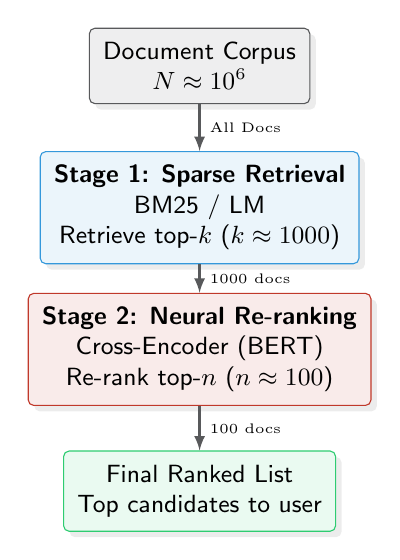
\begin{tikzpicture}[node distance=1.8cm]
    \node[infra] (corpus) {Document Corpus\\$N \approx 10^6$};
    \node[sparse, below of=corpus] (bm25) {\textbf{Stage 1: Sparse Retrieval}\\BM25 / LM\\Retrieve top-$k$ ($k \approx 1000$)};
    \node[rerank, below of=bm25] (rerank) {\textbf{Stage 2: Neural Re-ranking}\\Cross-Encoder (BERT)\\Re-rank top-$n$ ($n \approx 100$)};
    \node[hybrid, below of=rerank] (result) {Final Ranked List\\Top candidates to user};

    \draw[irArrowBase] (corpus) -- (bm25) node[midway, right, font=\tiny] {All Docs};
    \draw[irArrowBase] (bm25) -- (rerank) node[midway, right, font=\tiny] {1000 docs};
    \draw[irArrowBase] (rerank) -- (result) node[midway, right, font=\tiny] {100 docs};
\end{tikzpicture}

\end{center}
\end{column}
\end{columns}
\end{frame}

\begin{frame}{Why Two Stages?}
% \irStage{SYSTEM ARCHITECTURE}
\textbf{The pipeline separates the "wide net" retrieval from the "deep focus" ranking.}

\vspace{0.8em}
\begin{itemize}
    \item \textbf{Sparse (Recall)}: Microseconds per query. Metric: Recall@1000.
    \item \textbf{Neural (Precision)}: ~5ms scale per doc. Metric: NDCG@10.
    \item \textbf{Combined}: High precision search over an infinite corpus.
\end{itemize}\cpause

\vspace{1em}
\cpause
\begin{alertblock}{The Bounded Recall Problem}
If the sparse stage misses a document, the BERT stage can \textbf{never} score it. The first stage determines your performance upper-bound.
\end{alertblock}
\end{frame}

\begin{frame}{Comparing Pipeline Variants}
% \irStage{EVALUATION}
\begin{table}
\centering
\begin{tabular}{lcl}
\toprule
\textbf{Pipeline} & \textbf{NDCG@10} & \textbf{Latency} \\
\midrule
BM25 Only & 0.45 & 5 ms \\
BM25 + monoBERT & 0.55 & 500 ms \\
BM25 + RM3 + monoBERT & \textbf{0.57} & 520 ms \\
BM25 + monoT5-3B & \textbf{0.58} & 2 s \\
\bottomrule
\end{tabular}
\end{table}

\vspace{1em}
\cpause
\textbf{Insight:} Neural re-ranking provides the single largest gain in modern IR (~10 NDCG points).
\end{frame}

% \begin{frame}{What Neural Reranking Fixes}
% % \irStage{SYSTEM ARCHITECTURE}
% \begin{itemize}
%     \item \textbf{Vocabulary Mismatch:} \textit{heart attack} matches \textit{myocardial infarction}.
%     \item \textbf{Semantic Intent:} Understands \textit{how to...} vs \textit{definitions of...}
%     \item \textbf{Negation:} Understands \textit{countries \textbf{without} death penalty}.
% \end{itemize}\cpause

% \vspace{1em}
% \cpause
% \begin{alertblock}{When It Still Fails}
% If S1 recall is poor. If the document is longer than 512 tokens (truncation).
% \end{alertblock}
% \end{frame}


% ====================================================================
% NEW SECTION: TRAINING CROSS-ENCODERS
% ====================================================================
\section{Training Cross-Encoders in Practice}

\begin{frame}[plain]
\sectionpage
\end{frame}

\begin{frame}{The training data: MS MARCO}
% \irStage{TRAINING}
\textbf{Neural IR models are typically fine-tuned on the massive MS MARCO benchmark.}

\vspace{0.8em}
\begin{columns}
\begin{column}{0.55\textwidth}
\begin{itemize}
    \item \textbf{Scale}: 8.8M web passages and ~530k search queries.
    \item \textbf{Labels}: Sparse; usually only one relevant passage per query.
    \item \textbf{Dataset}: Collected from real Bing search logs and human editors.
\end{itemize}

\vspace{0.8em}
\begin{alertblock}{The Neural Catalyst}
\small This benchmark enabled the transition from lexical scoring to deep semantic ranking.
\end{alertblock}
\end{column}

\begin{column}{0.4\textwidth}
\begin{center}

\includegraphics[width=\textwidth]{figures/msmarco.pdf}
\end{center}
\end{column}
\end{columns}
\end{frame}


\begin{frame}[shrink=5]{Training Pipeline: Step by Step}
% \irStage{TRAINING}
\textbf{The training process iteratively refines the model's ability to rank relevant passages higher.}

\vspace{0.8em}
\begin{itemize}
    \item \textbf{Triples}: Train on $(q, d^+, d^-)$ tuples to learn relative relevance.
    \item \textbf{Loss}: Optimize Contrastive or Cross-Entropy loss functions.
    \item \textbf{Setup}: Typical training takes ~12--24 hours on one consumer GPU.
\end{itemize}\cpause

\vspace{0.5em}
\begin{center}
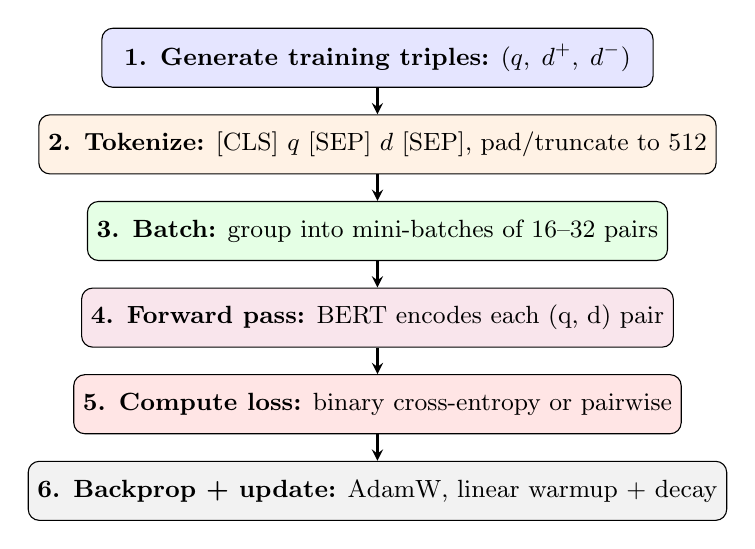
\begin{tikzpicture}[
    node distance=1.1cm,
    box/.style={rectangle, draw, rounded corners, minimum width=7cm, minimum height=0.75cm, align=center, font=\small},
    arrow/.style={->, thick, >=stealth}
]
    \node[box, fill=blue!10] (triples) {\textbf{1. Generate training triples:} $(q,\; d^+,\; d^-)$};
    \node[box, fill=orange!10, below of=triples] (tokenize) {\textbf{2. Tokenize:} [CLS] $q$ [SEP] $d$ [SEP], pad/truncate to 512};
    \node[box, fill=green!10, below of=tokenize] (batch) {\textbf{3. Batch:} group into mini-batches of 16--32 pairs};
    \node[box, fill=purple!10, below of=batch] (forward) {\textbf{4. Forward pass:} BERT encodes each (q, d) pair};
    \node[box, fill=red!10, below of=forward] (loss) {\textbf{5. Compute loss:} binary cross-entropy or pairwise};
    \node[box, fill=gray!10, below of=loss] (update) {\textbf{6. Backprop + update:} AdamW, linear warmup + decay};

    \draw[arrow] (triples) -- (tokenize);
    \draw[arrow] (tokenize) -- (batch);
    \draw[arrow] (batch) -- (forward);
    \draw[arrow] (forward) -- (loss);
    \draw[arrow] (loss) -- (update);
\end{tikzpicture}

\end{center}
\end{frame}


\begin{frame}{Fine-Tuning BERT for Ranking}
% \irStage{TRAINING}
\textbf{Supervised fine-tuning adapts the pre-trained model to specific ranking data.}

\vspace{0.8em}
\begin{itemize}
    \item \textbf{Pointwise}: Classify each pair (query, doc) as relevant or not.
    \item \textbf{Pairwise}: Train so $\text{score}(q, d^+) > \text{score}(q, d^-)$.
    \item \textbf{Data}: Usually requires large benchmarks like MS MARCO.
\end{itemize}

\vspace{1em}
\cpause
\begin{block}{Common Benchmarks}
\begin{itemize}
    \item \textbf{MS MARCO}: 530k queries with sparse (1 passage) labels.
    \item \textbf{TREC}: Smaller collections with dense, multi-level labels.
\end{itemize}
\end{block}
\end{frame}

\begin{frame}{MS MARCO: Sparse Labels Challenge}
% \irStage{TRAINING}
\textbf{Since labels are sparse, models must navigate a sea of unlabeled documents.}

\vspace{0.8em}
\begin{itemize}
    \item \textbf{False Negatives}: Many relevant documents are not labeled.
    \item \textbf{Bias}: We cannot treat all unlabeled docs as truly non-relevant.
    \item \textbf{Sampling}: How we choose the non-relevant pairs defines model quality.
\end{itemize}

\vspace{1em}
\cpause
\begin{exampleblock}{Implication}
Training on random negatives is insufficient. Models need challenging, "hard" negatives.
\end{exampleblock}
\end{frame}

\begin{frame}{Practice: Training BERT-base}
% \irStage{TRAINING}
\textbf{Fine-tuning requires careful initialization and small learning rates.}

\vspace{0.8em}
\begin{itemize}
    \item \textbf{Init}: Start from pre-trained weights (e.g., \texttt{bert-base-uncased}).
    \item \textbf{Length}: Must truncate query + doc to 512 sub-word tokens.
    \item \textbf{Schedule}: Learning rate $\approx 2 \times 10^{-5}$ for ~24 hours on one GPU.
\end{itemize}

\vspace{1em}
\cpause
\begin{alertblock}{Production Tip}
We are \textbf{refining} existing knowledge, not training from scratch!
\end{alertblock}
\end{frame}

\begin{frame}{Standard Models: monoBERT \& monoT5}
% \irStage{RE-RANKING}
\textbf{Two dominant architectures define the standard for neural re-ranking pipelines.}

\vspace{0.8em}
\begin{itemize}
    \item \textbf{monoBERT}: Encoder-only; uses the [CLS] token for classification.
    \item \textbf{monoT5}: Encoder-Decoder; uses generative prompts (``Is document relevant?'').
    \item \textbf{Choice}: monoT5 is often favored for its flexibility and accuracy.
\end{itemize}

\vspace{1em}
\cpause
\begin{exampleblock}{The SOTA Baseline}
Both models consistently outperform lexical methods by a large margin on TREC and MS MARCO.
\end{exampleblock}
\end{frame}


\begin{frame}{Comparison: monoBERT vs. monoT5}
% \irStage{RE-RANKING}
\textbf{While both are effective, they differ in architecture and training objectives.}

\vspace{0.8em}
\begin{itemize}
    \item \textbf{monoBERT}: Faster inference; trained via classification.
    \item \textbf{monoT5}: More flexible; trained via sequence-to-sequence generation.
    \item \textbf{Trade-off}: T5's generative approach often yields slightly higher accuracy.
\end{itemize}

\vspace{1em}
\cpause
\begin{table}
\centering
\small
\begin{tabular}{lll}
\toprule
\textbf{Feature} & \textbf{monoBERT} & \textbf{monoT5} \\
\midrule
Architecture & Encoder-only & Encoder-Decoder \\
Objective & Classification & Text Generation \\
Inference & Slightly faster & Slightly slower \\
\bottomrule
\end{tabular}
\end{table}
\end{frame}


% \begin{frame}{ColBERT: Late Interaction}
% % \irStage{REPRESENTATION}
% \textbf{ColBERT enables token-level matching while maintaining high search efficiency.}

% \vspace{0.8em}
% \begin{itemize}
%     \item \textbf{Independence}: Query and Doc tokens are encoded separately.
%     \item \textbf{Interaction}: Deep matching occurs only at the final MaxSim layer.
%     \item \textbf{Scalability}: Enables sub-millisecond search over full corpora.
% \end{itemize}\cpause

% % \vspace{0.5em}
% % \begin{center}
% % 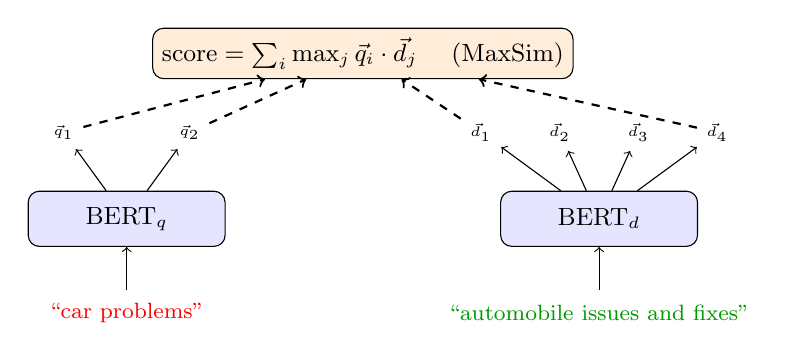
\begin{tikzpicture}[
    box/.style={rectangle, draw, rounded corners, fill=blue!10, minimum height=0.7cm, align=center, font=\small},
    arrow/.style={->, thick}
]
    \node[box, minimum width=2.5cm] (bq) at (0, 1.5) {BERT$_q$};
    \node[box, minimum width=2.5cm] (bd) at (6, 1.5) {BERT$_d$};

    \node[font=\footnotesize, red] at (0, 0.3) {``car problems''};
    \node[font=\footnotesize, green!60!black] at (6, 0.3) {``automobile issues and fixes''};

    \node[font=\tiny] (e1) at (-0.8, 2.6) {$\vec{q}_1$};
    \node[font=\tiny] (e2) at (0.8, 2.6) {$\vec{q}_2$};

    \node[font=\tiny] (d1) at (4.5, 2.6) {$\vec{d}_1$};
    \node[font=\tiny] (d2) at (5.5, 2.6) {$\vec{d}_2$};
    \node[font=\tiny] (d3) at (6.5, 2.6) {$\vec{d}_3$};
    \node[font=\tiny] (d4) at (7.5, 2.6) {$\vec{d}_4$};

    \draw[arrow, thin] (0, 0.6) -- (bq);
    \draw[arrow, thin] (6, 0.6) -- (bd);

    \draw[arrow, thin] (bq) -- (e1);
    \draw[arrow, thin] (bq) -- (e2);
    \draw[arrow, thin] (bd) -- (d1);
    \draw[arrow, thin] (bd) -- (d2);
    \draw[arrow, thin] (bd) -- (d3);
    \draw[arrow, thin] (bd) -- (d4);

    \node[rectangle, draw, fill=orange!15, rounded corners, font=\small] (maxsim) at (3, 3.6) {$\text{score} = \sum_i \max_j \vec{q}_i \cdot \vec{d}_j$ \quad (MaxSim)};

    \draw[arrow, dashed] (e1) -- (maxsim);
    \draw[arrow, dashed] (e2) -- (maxsim);
    \draw[arrow, dashed] (d1) -- (maxsim);
    \draw[arrow, dashed] (d4) -- (maxsim);
\end{tikzpicture}

% % \end{center}
% \end{frame}


% \begin{frame}{ColBERT: Late Interaction}
% % \irStage{REPRESENTATION}
% \textbf{ColBERT enables token-level matching while maintaining high search efficiency.}

% \vspace{0.8em}

% \begin{center}
% 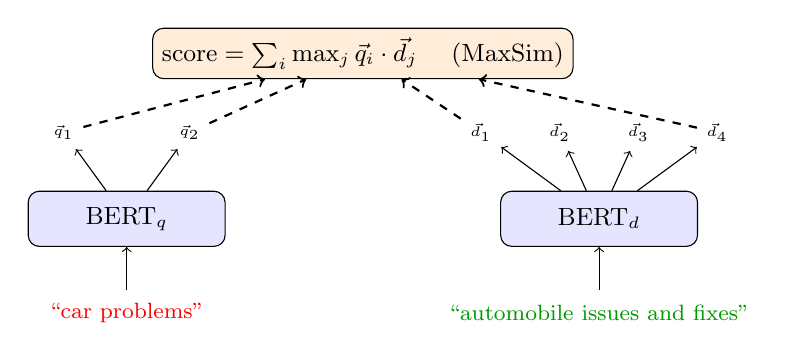
\begin{tikzpicture}[
    box/.style={rectangle, draw, rounded corners, fill=blue!10, minimum height=0.7cm, align=center, font=\small},
    arrow/.style={->, thick}
]
    \node[box, minimum width=2.5cm] (bq) at (0, 1.5) {BERT$_q$};
    \node[box, minimum width=2.5cm] (bd) at (6, 1.5) {BERT$_d$};

    \node[font=\footnotesize, red] at (0, 0.3) {``car problems''};
    \node[font=\footnotesize, green!60!black] at (6, 0.3) {``automobile issues and fixes''};

    \node[font=\tiny] (e1) at (-0.8, 2.6) {$\vec{q}_1$};
    \node[font=\tiny] (e2) at (0.8, 2.6) {$\vec{q}_2$};

    \node[font=\tiny] (d1) at (4.5, 2.6) {$\vec{d}_1$};
    \node[font=\tiny] (d2) at (5.5, 2.6) {$\vec{d}_2$};
    \node[font=\tiny] (d3) at (6.5, 2.6) {$\vec{d}_3$};
    \node[font=\tiny] (d4) at (7.5, 2.6) {$\vec{d}_4$};

    \draw[arrow, thin] (0, 0.6) -- (bq);
    \draw[arrow, thin] (6, 0.6) -- (bd);

    \draw[arrow, thin] (bq) -- (e1);
    \draw[arrow, thin] (bq) -- (e2);
    \draw[arrow, thin] (bd) -- (d1);
    \draw[arrow, thin] (bd) -- (d2);
    \draw[arrow, thin] (bd) -- (d3);
    \draw[arrow, thin] (bd) -- (d4);

    \node[rectangle, draw, fill=orange!15, rounded corners, font=\small] (maxsim) at (3, 3.6) {$\text{score} = \sum_i \max_j \vec{q}_i \cdot \vec{d}_j$ \quad (MaxSim)};

    \draw[arrow, dashed] (e1) -- (maxsim);
    \draw[arrow, dashed] (e2) -- (maxsim);
    \draw[arrow, dashed] (d1) -- (maxsim);
    \draw[arrow, dashed] (d4) -- (maxsim);
\end{tikzpicture}

% \end{center}
% \end{frame}

% \begin{frame}{ColBERT: Why It Matters}
% % \irStage{REPRESENTATION}
% \textbf{Late interaction provides near-optimal accuracy with retrieval-time speed.}

% \vspace{0.8em}
% \begin{itemize}
%     \item \textbf{MaxSim}: Aggregates token-level cosine similarities across the query.
%     \item \textbf{Speed}: ~20ms scale vs ~500ms for Cross-Encoders.
%     \item \textbf{Efficiency}: Pre-computes and stores document token embeddings.
% \end{itemize}\cpause

% \vspace{0.5em}
% \begin{table}
% \centering
% \scriptsize
% \begin{tabular}{lccc}
% \toprule
%  & \textbf{Cross-Encoder} & \textbf{ColBERT} & \textbf{Bi-Encoder} \\
% \midrule
% Interaction & Full (all layers) & Late (token-level) & Dot product only \\
% Pre-computation & \textcolor{irRerank}{\texttimes} No & \textcolor{irHybrid}{\checkmark} Yes (token) & \textcolor{irHybrid}{\checkmark} Yes (single) \\
% Latency & ~500ms & ~20ms & ~10ms \\
% Storage & N/A & ~10--50 KB/doc & ~3 KB/doc \\
% \bottomrule
% \end{tabular}
% \end{table}
% \end{frame}


\begin{frame}{Common Training Pitfalls}
% \irStage{TRAINING}
\begin{itemize}
    \item \textbf{Overfitting:} Neural rankers overfit MS MARCO quickly. Stop at 2--3 epochs.
    \item \textbf{Catastrophic Forgetting:} Use small learning rates ($< 3 \times 10^{-5}$) and warmup.
    \item \textbf{Weak Negatives:} Random samples are too easy. Use BM25 hard negatives.
\end{itemize}\cpause
\end{frame}

\begin{frame}[fragile,shrink=10]{Implementation (Hugging Face)}
% \irStage{TRAINING}
\begin{lstlisting}[language=Python]
model = AutoModelForSequenceClassification.from_pretrained("bert-base-uncased")
tokenizer = AutoTokenizer.from_pretrained("bert-base-uncased")

# Training args
args = TrainingArguments(
    per_device_train_batch_size=16,
    learning_rate=2e-5,
    num_train_epochs=3,
    fp16=True
)
# Trainer handles batching, eval, and optimization
trainer = Trainer(model=model, args=args, train_dataset=ds)
trainer.train()
\end{lstlisting}
\end{frame}

% % ====================================================================
% % SECTION 5: HANDS-ON
% % ====================================================================
% \section{Hands-On: Neural Pipelines}

% \begin{frame}[fragile]{Setup: Loading Models}
% \irStage{PRACTICE}
% \begin{lstlisting}[language=Python, basicstyle=\small\ttfamily]
% import pyterrier as pt
% from pyterrier_t5 import MonoT5ReRanker

% # BM25 baseline (Lecture 3)
% bm25 = pt.BatchRetrieve(index, wmodel="BM25")

% # Load monoT5 re-ranker
% monoT5 = MonoT5ReRanker()
% \end{lstlisting}
% \end{frame}

% \begin{frame}[fragile]{Exercise 1: The Reranking Pipeline}
% \irStage{PRACTICE}
% \begin{lstlisting}[language=Python, basicstyle=\small\ttfamily]
% # Stage 1: BM25 retrieves top 100
% # Stage 2: monoT5 re-ranks
% pipeline = (bm25 % 100) >> monoT5

% # Evaluate
% pt.Experiment(
%     [bm25, pipeline],
%     topics, qrels,
%     eval_metrics=["map", "ndcg_cut_10"],
%     names=["BM25", "BM25 + monoT5"]
% )
% \end{lstlisting}
% \end{frame}

% \begin{frame}{Exercise 2: Analyzing Improvements}
% \irStage{PRACTICE}
% \begin{itemize}
%     \item Find a query where \textbf{monoT5 >> BM25}.
%     \item Inspect the top Docs.
%     \item \textbf{Question:} Why did BM25 fail? (Mismatch? Intent?)
% \end{itemize}\cpause
% \end{frame}

% \begin{frame}{Practice: Depth vs. Accuracy}
% \irStage{PRACTICE}
% \textbf{How many documents should we re-rank for the best performance?}

% \vspace{0.8em}
% \begin{itemize}
%     \item \textbf{top-10}: Extremely fast, but minimal recall coverage.
%     \item \textbf{top-100}: Best quality/latency trade-off \textcolor{irHybrid}{\checkmark}.
%     \item \textbf{top-1000}: Diminishing returns; latency becomes too high.
% \end{itemize}\cpause

% \vspace{1em}
% \cpause
% \begin{exampleblock}{Conclusion}
% Re-ranking beyond 100--200 documents rarely improves top-10 metrics, but increases latency linearly.
% \end{exampleblock}
% \end{frame}

% \begin{frame}{Student Exercise: Analyze (15 min)}
% \irStage{PRACTICE}
% \begin{enumerate}
%     \item Find a query where \textbf{monoT5} moves a relevant doc from pos 50 to pos 1.
%     \item Find a query where the relevant doc is \textbf{not in the top 100}.
%     \item \textbf{Discuss:} Can the re-ranker help in Case 2?
% \end{enumerate}
% \end{frame}


% ====================================================================
% SECTION 6: CONNECTIONS
% ====================================================================
\section{Connections and Summary}

\begin{frame}[plain]
\sectionpage
\end{frame}

\begin{frame}{The Representation Spectrum}
% \irStage{SUMMARY}
\textbf{Text representations evolved from sparse matching to deep semantic interaction.}

\vspace{0.8em}
\begin{itemize}
    \item \textbf{Sparse}: High scalability, zero semantics (Exact-match bottleneck).
    \item \textbf{Dense}: Good semantics, high scalability via ANN (Retrieval).
    \item \textbf{Neural}: Deepest interaction, lowest scalability (Re-ranking).
\end{itemize}\cpause

\vspace{0.5em}
\begin{center}
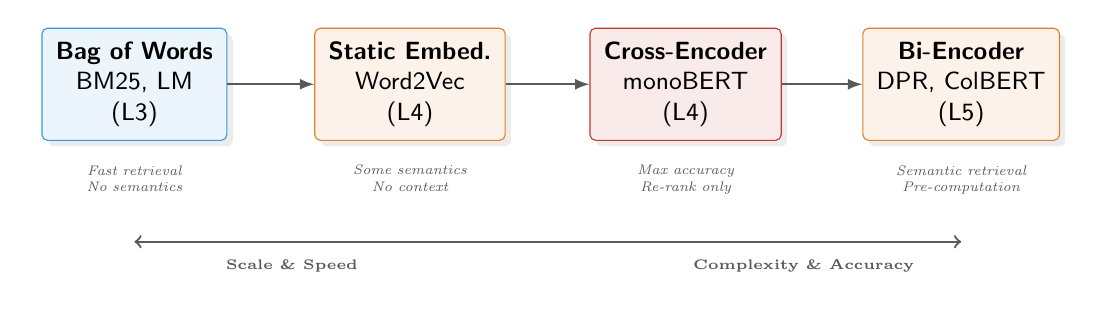
\begin{tikzpicture}
    % Spectrum Nodes
    \node[sparse] (bow) at (0, 0) {\textbf{Bag of Words}\\BM25, LM\\(L3)};
    \node[dense] (static) at (3.5, 0) {\textbf{Static Embed.}\\Word2Vec\\(L4)};
    \node[rerank] (cross) at (7, 0) {\textbf{Cross-Encoder}\\monoBERT\\(L4)};
    \node[dense] (bi) at (10.5, 0) {\textbf{Bi-Encoder}\\DPR, ColBERT\\(L5)};

    % Connections
    \draw[irArrowBase] (bow) -- (static);
    \draw[irArrowBase] (static) -- (cross);
    \draw[irArrowBase] (cross) -- (bi);

    % Captions
    \node[below=0.2cm of bow, irLabel] {Fast retrieval\\No semantics};
    \node[below=0.2cm of static, irLabel] {Some semantics\\No context};
    \node[below=0.2cm of cross, irLabel] {Max accuracy\\Re-rank only};
    \node[below=0.2cm of bi, irLabel] {Semantic retrieval\\Pre-computation};

    % Axis
    \draw[<->, thick, irInfra] (0, -2) -- (10.5, -2);
    \node[font=\tiny\bfseries, irInfra, anchor=north] at (2, -2.1) {Scale \& Speed};
    \node[font=\tiny\bfseries, irInfra, anchor=north] at (8.5, -2.1) {Complexity \& Accuracy};
\end{tikzpicture}

\end{center}
\end{frame}


\end{document}